\documentclass{article}
\usepackage{amssymb, amsmath, amsthm}
\usepackage[margin=1in]{geometry}
\usepackage{verbatim}
\usepackage{graphicx}
\usepackage{hyperref} % \url \href
\usepackage{docmute}

\newtheorem{definition}{Definition}
\newtheorem{theorem}{Theorem}
\newcommand{\heff}{\mathbb{H}^{\text{eff}}}
\newcommand{\pfrac}[2]{\frac{\partial #1}{\partial #2}}

\newcommand{\MO}{\textbf{MO}}
\newcommand{\AO}{\textbf{AO}}

\newcommand{\huptb}{\text{H}_0}
\newcommand{\order}[2]{#1^{(#2)}}
\newcommand{\statebra}[1]{\langle #1 |}
\newcommand{\stateket}[1]{| #1 \rangle}

\begin{document}

\section{Molecular Orbitals in Conjugated System and Solids}
\subsection{Conjugated System}
Conjugated system\footnote{\url{https://en.wikipedia.org/wiki/Conjugated_system}} 
refer to systems consists of connected $p$ orbitals with delocalized electrons in a molecular. 
Let's consider $N$ $\pi$ orbitals along a chain with nearest neighbor interaction and 
we further assume that their orbitals are non-overlapping so that the matrix 
element is $S_{\mu\nu} = \delta_{\mu\nu}$. 
The reason that we choose $\pi$ orbital system is because the small orbital overlap in this 
situation, as compared to the head to head sigma interactions. 
Let the energy of the $p$ orbital itself to be $\alpha$
and the nearest neighbor interaction $\beta < 0$, the secular equation can be reduced to 
an eigen-equation:
\begin{equation}
    H^{AO} \mathbf{C}_i = \varepsilon_i \mathbf{C}_i
\end{equation}
where the form of the Hamiltonian is like:
\begin{equation}
    H^{AO}_{N=3} = \left(\begin{matrix}
        \alpha & \beta & 0 \\ 
        \beta & \alpha & \beta \\ 
        0 & \beta & \alpha 
    \end{matrix}\right)
\end{equation}
The solution of the eigen-equation is given by:
\begin{align}
    \varepsilon_j &= \alpha + 2 \beta \cos\frac{j\pi}{N+1} \\ 
    c_{\mu j} &= \left(\frac{2}{N+1}\right)^{1/2} \sin\left(\frac{\mu j\pi}{N+1}\right) 
\end{align}
where $j$ index\footnote{$j$ is used instead of $i$ to avoid confusion with imaginary number $i$} 
the obtained molecular orbital and $\mu$ index the consistuting atomic orbitals. 

The importance of the factor $N+1$ can be shown as follows: we subsitute the solution into the 
eigen-equation:
\begin{equation}
    \sum_{\nu} H_{\mu\nu} C_{\nu j} = H_{\mu\mu-1} C_{\mu-1 j} + H_{\mu\mu} C_{\mu j} + H_{\mu\mu+1} C_{\mu+1 j} = \varepsilon_j C_{\mu j}
\end{equation}
where we use the fact that the summation is restricted to the nearest neighbors only. Using the 
solution, we obtain the expression:
\begin{align}
    &\left(\alpha + 2 \beta \cos\frac{j\pi}{N+1}\right) \sin\frac{\mu j\pi}{N+1} \\
    &= \alpha \sin\frac{\mu j\pi}{N+1} + 2 \beta \cos\frac{j\pi}{N+1} \sin\frac{\mu j\pi}{N+1} \\ 
    &= \left[\beta\cdot \sin\frac{(\mu-1) j\pi}{N+1}  \right. 
     \left. + \alpha\cdot\sin\frac{\mu j\pi}{N+1}  + \beta \cdot \sin \frac{(\mu+1) j\pi}{N+1}\right] 
\end{align} 
where the common normalization factor $(2/(N+1))^{1/2}$ is removed. The term with $\alpha$ are the same on both side 
so we only need to show that:
\begin{equation}
    2 \beta \cos\frac{j\pi}{N+1} \sin\frac{\mu j\pi}{N+1} 
    = \beta\cdot \sin\left( \frac{\mu j\pi}{N+1} - \frac{j\pi}{N+1} \right) 
    + \beta\cdot \sin\left( \frac{\mu j\pi}{N+1} + \frac{j\pi}{N+1} \right)
\end{equation}
For $1 \leq \mu \leq N$. We can consider three cases: 
For $\mu = 1$, the right hand side become:
\begin{equation}
    \beta\cdot \sin\left( \frac{j\pi}{N+1} + \frac{j\pi}{N+1} \right) 
    = 2 \beta \sin \frac{j\pi}{N+1} \cos \frac{j\pi}{N+1} 
\end{equation}
since $\sin(2\alpha) = 2\sin\alpha\cos\alpha$. 
For $1 < \mu < N$, we can similarly show that the equality is true with 
$\sin(\alpha \pm \beta) = \sin\alpha\cos\beta \pm \sin\beta\cos\alpha$. 
The effect of factor $N+1$ is shown when $\mu = N$, in which case we have, for the right hand side:
\begin{align}
    \beta\cdot \sin\left( \frac{N j\pi}{N+1} - \frac{j\pi}{N+1} \right) 
    &= \beta \left( \sin\frac{N j\pi}{N+1}\cos\frac{j\pi}{N+1} - \cos\frac{N j\pi}{N+1}\sin\frac{j\pi}{N+1}  \right) \\ 
    &= \beta \left( \sin\frac{N j\pi}{N+1}\cos\frac{j\pi}{N+1} - \cos\left(1 - \frac{j\pi}{N+1}\right)\sin\left(1 - \frac{Nj\pi}{N+1}\right)  \right) \\ 
    &=2 \beta \sin\frac{N j\pi}{N+1}\cos\frac{j\pi}{N+1}
\end{align}
If we have $N$ instead of $N+1$, then the last situation will not be correct.

\subsection{Cyclic systems}
Let's now consider the case of cyclic system with single $s$ orbitals on each site and nearest neighbor interaction. 
This situation is close to that in solids with periodic boundary condition. The solution is now given by:
\begin{align}
    \label{E:cyclic_system_energy}
    \varepsilon_j &= \alpha + 2 \beta \cos\frac{j\pi}{N} \\ 
    c_{\mu j} &= \frac{1}{\sqrt{N}} \exp \frac{2\pi i \cdot j (\mu-1)}{N} 
\end{align}
where we take the index of $j$ to start from 0. 
The energy level obtained in such approach can be graphically shown as in figure \ref{F:cyclic_energy} 
where we can always find a single degenerate state at energy $\alpha + 2 \beta$. If $N$ is even, we have 
another single degenerate state with energy $\alpha - 2 \beta$. All the other states are doubly degenerate. 
\begin{figure}[h!]
    \centering
    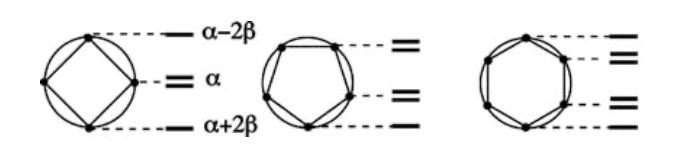
\includegraphics[width=3in]{figures/F_cyclic_energy.png}
    \caption{Graphical illustration of cyclic energy}
    \label{F:cyclic_energy}
\end{figure}
This is true for cyclic groups $C_n$ if we check their character tables, as shown for group $C_4$, $C_5$ and 
$C_6$ in figure \ref{F_cyclic_group_table}

\begin{figure}[h!]
    \centering
    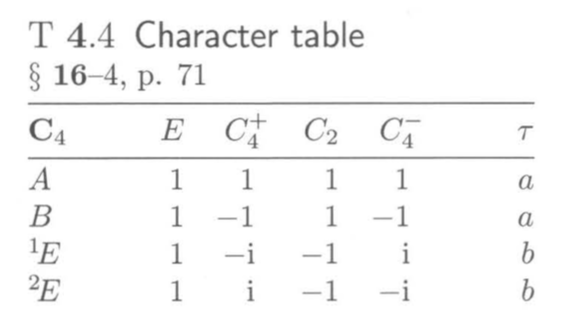
\includegraphics[width=3in]{figures/F_C4.png}
    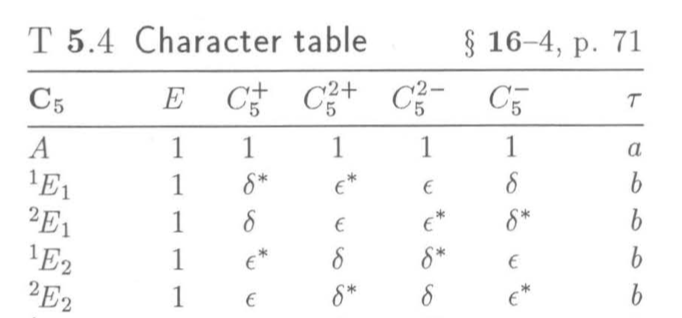
\includegraphics[width=3in]{figures/F_C5.png}
    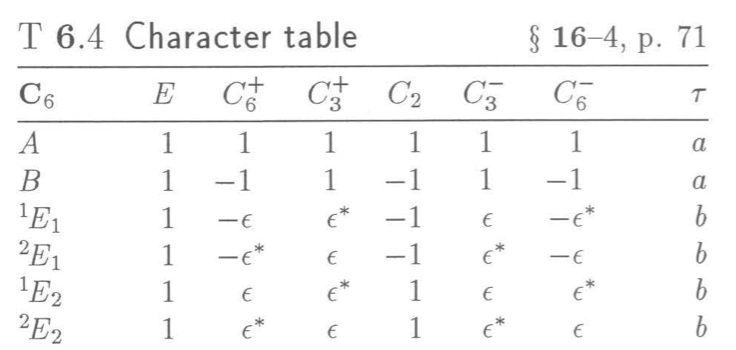
\includegraphics[width=3in]{figures/F_C6.png}
    \caption{Character tables for cyclic groups}
    \label{F_cyclic_group_table}
\end{figure}

\subsection{Solids}
Let's consider as example, only the one dimension chain that extend infinitely in one direction but are joined 
at the two end, so that the situation is similar to that of the cyclic system. 
We use the interaction parameter similar to that of the cyclic system so that the energy can still be 
expressed using equation \eqref{E:cyclic_system_energy}. However, we use the vector $k$:
\begin{equation}
    k = \frac{2\pi j}{Na}
\end{equation}
so that the energy and wavefunction can be expressed as:
\begin{align}
    \varepsilon_j &= \alpha + 2 \beta \cos ka \\ 
    c_{\mu j} &= \frac{1}{\sqrt{N}} e^{ik(\mu-1) a} = \frac{1}{\sqrt{N}} e^{ikR_{\mu}}
\end{align}
where now each wavefunction $\chi_{\mu}$ is a considered to be in the $\mu$th cell. 

Let's now take into account the overlap matrix $S$. The eigenstates in solids are given 
by functions that satisfy the bloch condition: $\phi_k(r+l) = e^{ikl} \phi_k(r)$ where $l$ 
is a lattice vector. 
\begin{align}
    \psi_j^k(r) &= \sum_{\mu}c^k_{\mu j}\phi_{\mu}^k(r) \\ 
    \phi_{\mu}^k(r) &= \frac{1}{\sqrt{N}} \sum_p e^{ikR_p} \chi_{\mu}(r - R_p)
\end{align}
we can verify:
\begin{align}
    \psi_j^k(r+l) &= \frac{1}{\sqrt{N}} \sum_{\mu} c^k_{\mu j} \sum_p e^{ikR_p} \chi_{\mu}(r - (R_p - l)) \\ 
    &= \frac{1}{\sqrt{N}} \sum_{\mu} c^k_{\mu j} \sum_{p'} e^{ik(R_{p'}+l)} \chi_{\mu}(r - R_{p'}) \\ 
    &= e^{ikl} \phi_j^k(r)
\end{align}
Now, let's solve the eigenequation:
\begin{align}
    H \stateket{ \psi_j^k } &= \varepsilon_j^k \stateket{ \psi_j^k } \\ 
    \frac{1}{N} \sum_{\mu} c^k_{\mu j} \sum_{pp'} e^{ik(R_p - R_{p'})} \statebra{\chi_{\nu,R_{p'}}} H \stateket{\chi_{\mu,R_p}}
    &= \frac{1}{N}  \varepsilon_j^k \sum_{\mu} c^k_{\mu j} \sum_{pp'} e^{ik(R_p - R_{p'})} \statebra{\chi_{\nu,R_{p'}}} \chi_{\mu,R_p} \rangle \\ 
    \sum_{\mu} c^k_{\mu j} H_{\nu\mu}^k &= \varepsilon_j^k \sum_{\mu} c^k_{\mu j} S_{\nu\mu}^k \\ 
    \mathbf{H}^k \mathbf{C}_{j}^k &= \varepsilon_j^k \mathbf{H}^k \mathbf{S}_{j}^k
\end{align}
where we multiplied $\statebra{\phi_{\mu}^k}$ on the left for the second relationship. The final equation 
is the tight binding secular equation in solids, where 
\begin{align}
    H_{\nu\mu}^k = \sum_p e^{ikR_p} \statebra{\chi_{\nu,R_0}} H \stateket{\chi_{\mu,R_p}} \\ 
    S_{\nu\mu}^k = \sum_p e^{ikR_p} \statebra{\chi_{\nu,R_0}} \chi_{\mu,R_p} \rangle
\end{align}

\subsection{Interpretation of band dispersion with avoided crossing}
In this section, we point out the complication introduced by avoided crossing in 
Interpretation of band dispersion with a $sp$ one dimensional chain along $z$ direction 
with total 4 bands.
The case of $p_x$, $p_y$ and $s$ follows the above discussion. At the zone center, $k=0$ and we 
have the lowest energy $\varepsilon_{k=0} = \alpha + 2\beta$ and at the zone edge where $k = \pi/a$ 
we have the highest energy $\varepsilon_{k=\pi/a} = \alpha - 2\beta$. $\beta$ is defined to be a 
negative value. Therefore, these bands \emph{run up} in band dispersion along $\Gamma-X$. 
In terms of energy position, $p_x$ and $p_y$ bands are degenerate and located higher 
in energy compared to the $s$ bands. For $p_z$ band, its dispersion $runs down$, as can be 
seen from figure \ref{F:pz}. Furthermore, due to strong $\sigma$ interaction, the band is very dispersive. 

\begin{figure}[h!]
    \centering
    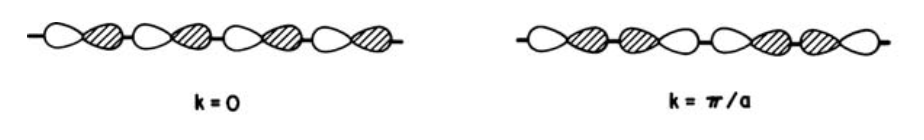
\includegraphics[width=3in]{figures/F_pz.png}
    \caption{Wavefunction of the $p_z$ band at $k=0$ and $k=\pi/a$}
    \label{F:pz}
\end{figure}

It is clear that at both $k=0$ and $k=\pi/a$, these four bands cannot interact with each other 
because of the symmetry of the wavefunction: on each site the overlap integral vanish. However, 
this is not so on the path between $\Gamma$ and $X$ points. Along the line, $p_x$ and $p_y$ 
does not interact but $p_z$ and $s$ band does. Interaction created avoided crossing, as shown 
by the figure \ref{F:avoid_interaction}.

\begin{figure}[h!]
    \centering
    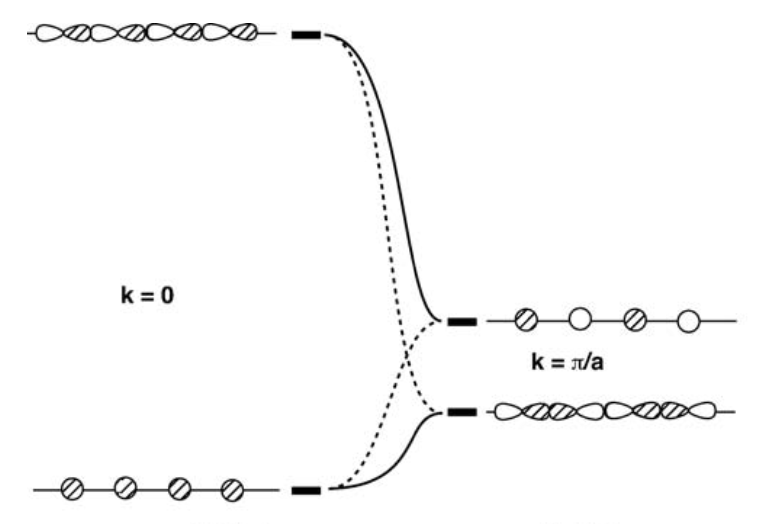
\includegraphics[width=2in]{figures/F_avoid_interaction_spz.png}
    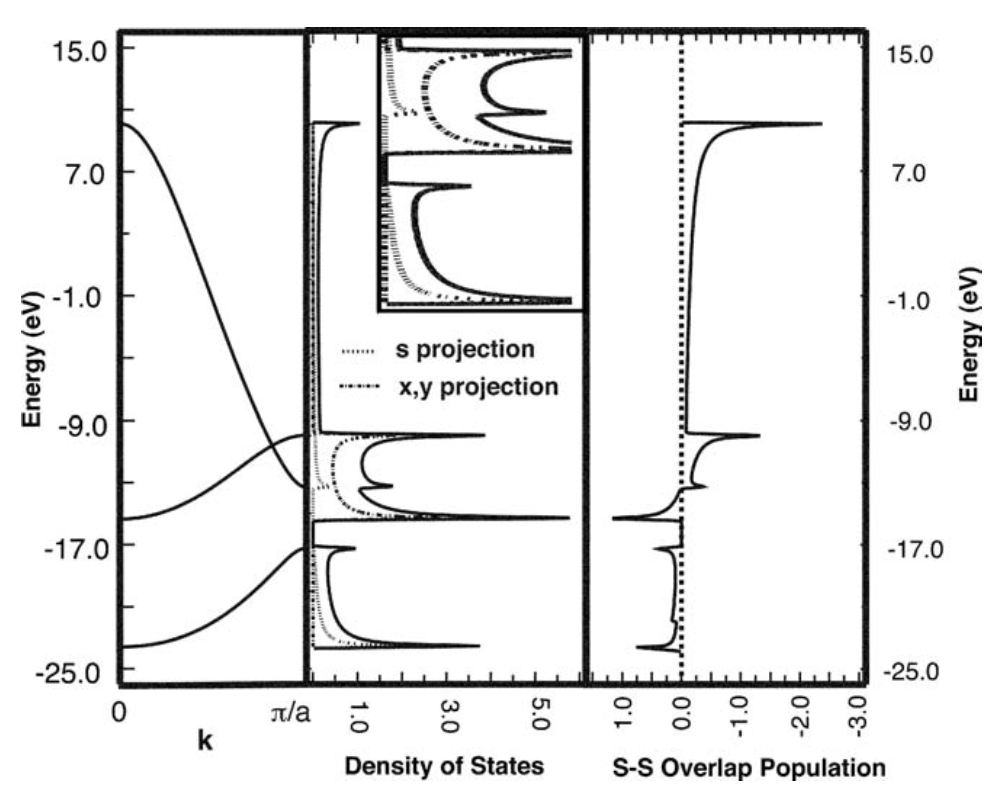
\includegraphics[width=3in]{figures/F_avoid_interaction_dispersion.png}
    \caption{Avoid interaction in band dispersion}
    \label{F:avoid_interaction}
\end{figure}

It is now clear that although in the band dispersion, the $s$ band running up and $p_z$ band 
running down seems to be formed purely by $s$ and $p_z$ themselves, they are actually mixed. 
We use the lower $s$ band as an example for the consequence for the avoided crossing:
\begin{enumerate}
    \item Due to the mixing, the density of state of the upper part of the band is mainly $p_z$ character, and 
    \item Both the top and bottum of the band are $bonding$. This is opposite to the isolated case (for example $p_x$) where 
          the bottum of the band is bonding and the top are antibonding. 
\end{enumerate}

\end{document}
